% !TeX program = pdflatex
% NOMS 2027 working manuscript. IEEE conference format (official template, 2024-06-28).
% Compile this file directly using pdfLaTeX.
\documentclass[conference]{IEEEtran}
% \IEEEoverridecommandlockouts % Enable only if a funding footnote requires it.
\usepackage{cite}
\usepackage{amsmath,amssymb,amsfonts}
\usepackage{algorithmic}
\usepackage{graphicx}
\usepackage{textcomp}
\usepackage{xcolor}
\def\BibTeX{{\rm B\kern-.05em{\sc i\kern-.025em b}\kern-.08em
    T\kern-.1667em\lower.7ex\hbox{E}\kern-.125emX}}

% Manuscript-specific semantic macros (do not change IEEE page geometry or fonts).
\newcommand{\QUERY}{\textsf{QUERY}}
\newcommand{\REFRESH}{\textsf{REFRESH}}
\newcommand{\SKIP}{\textsf{SKIP}}
\newcommand{\STOP}{\textsf{STOP}}
\newcommand{\TODO}[1]{\textit{[Draft: #1]}}

\title{Intent-Aware Sequential Resource Discovery\\under Uncertain Domain Knowledge}

\author{\IEEEauthorblockN{D\'aniel Ficzere\IEEEauthorrefmark{1}\IEEEauthorrefmark{2},
Attila Frank\'o\IEEEauthorrefmark{1},
Gergely Holl\'osi\IEEEauthorrefmark{1},
P\'al Varga\IEEEauthorrefmark{1},
J\'ozsef B\'ir\'o\IEEEauthorrefmark{1}}
\IEEEauthorblockA{\IEEEauthorrefmark{1}Department of Telecommunications and Artificial Intelligence,\\
Budapest University of Technology and Economics, Budapest, Hungary}
\IEEEauthorblockA{\IEEEauthorrefmark{2}AI \& IIoT Division, AITIA International Inc., Budapest, Hungary}
}
\begin{document}
\maketitle

\begin{abstract}
Intent-based management in federated edge environments must discover
resources using partial, aggregated, and possibly stale domain knowledge.
We investigate the joint choice of where to search, when to refine
information, and when further discovery can be avoided under an explicit
residual-risk constraint. A sequential model combines exact resource
queries, imperfect summary refreshes, domain skipping, and stopping.
Structural observations motivate an intent-aware one-step rollout and a
polynomial-time skip-aware continuation heuristic.
This manuscript is a \emph{working structure}: formal claims, numerical
results, and the final performance evidence will be inserted after validation.
\end{abstract}

\begin{IEEEkeywords}
intent-based networking, resource discovery, network management,
sequential decision making, value of information, edge computing
\end{IEEEkeywords}

\section{Introduction}
\label{sec:intro}
Federated edge and network-management infrastructures distribute
resources across independently managed domains. An intent defines
requirements such as compute capacity, memory, and latency, yet a
management controller may have only summary-level knowledge of the
actual resource availability. Obtaining an exact answer incurs
communication or operational cost; refreshing a domain summary can be
cheaper but imperfect.

\paragraph{Problem statement.}
We seek a policy that minimizes expected discovery cost while bounding
the probability of terminating without finding an available suitable
resource. The management decision jointly concerns \emph{where to
query}, \emph{whether to refresh}, and \emph{whether to skip or stop}.

\paragraph{Planned contributions.}
\begin{itemize}
\item \textbf{C1 -- Decision model:} a unified \QUERY/\REFRESH/\SKIP/\STOP
formulation with intent-conditioned beliefs and an explicit
residual-risk constraint.
\item \textbf{C2 -- Structural results:} query and fixed-module ordering,
screening, deferred refresh, ordering probes, and precisely qualified
pruning rules.
\item \textbf{C3 -- Algorithm and evaluation:} a scalable
IA-OSR-PSA1 rollout compared with exact Bellman optimization and
relevant discovery baselines.
\end{itemize}
% TODO: replace with verified novelty language and paper roadmap.

\section{Related Work}
\label{sec:related}
\TODO{Synthesize: intent-to-resource mapping; semantic and distributed
service discovery; aggregated domain summaries; freshness-aware source
selection; active information acquisition and value of information.}

% TODO: insert verified references and bibliographic entries.
% Avoid claiming that any individual component (e.g., Bayesian updates or
% age-aware source selection) is new; emphasize the joint sequential decision.

\section{System Model and Problem Formulation}
\label{sec:model}
\subsection{Domains, intents, and beliefs}
Let $\mathcal D=\{D_1,\ldots,D_N\}$ denote the candidate domains.
For intent $I$, write
\begin{equation}
 p_i(I,t)=\Pr\bigl(X_i(I,t)=1\mid K_i(t)\bigr),
 \label{eq:belief}
\end{equation}
where $K_i(t)$ is persistent domain knowledge and $X_i(I,t)$ indicates
that a feasible resource exists in $D_i$. For the single-intent,
single-epoch analysis we write $p_i$. A class-based construction may
supply $p_i$, but detailed estimation and latent-state extensions are
outside the main paper.

\subsection{Information acquisition and stopping}
An exact query $Q_i$ has cost $q_i>0$; an imperfect refresh $R_i$
has cost $r_i>0$, sensitivity $\alpha_i$, and specificity $\beta_i$.
The positive observation probability is
\begin{equation}
 g_i=p_i\alpha_i+(1-p_i)(1-\beta_i),\quad h_i=1-g_i.
\end{equation}
Bayesian updating yields $p_i^+$ or $p_i^-$ following the observation.
At most one refresh per domain is allowed; a successful exact query
terminates discovery. Domains are independent in the baseline model.

The risk tolerance $\varepsilon$ bounds the residual probability that
an unexamined or skipped domain still contains a suitable resource.
The distinction between irrevocably skipped domains and fully
resolved queries must be retained in the decision state.

\subsection{Sequential optimization}
Let $s$ record unresolved domains, beliefs, refresh outcomes, skipped
risk, and admissible future actions. The benchmark is the Bellman
recursion
\begin{equation}
 V^\star(s)=\min_{a\in\mathcal A(s)}
 \bigl\{c(a)+\mathbb E[V^\star(s')\mid s,a]\bigr\}.
 \label{eq:bellman}
\end{equation}
\TODO{Provide exact state encoding and admissibility conditions; give a
small, auditable running edge/GPU example.}

\section{Structural Insights}
\label{sec:structural}
\subsection{Optimal query and fixed-module ordering}
For query-only search, domains are processed in nondecreasing order of
\begin{equation}
 J_i^Q=\frac{q_i}{p_i}.
\end{equation}
The same adjacent-interchange argument extends to fixed modules with
expected internal cost $c_i$ and termination probability $s_i$, using
$c_i/s_i$ under the relevant state-invariance assumptions.

\subsection{Screening and deferred refresh}
A screening module refreshes a domain and performs an exact query only
following a positive signal; a negative result may authorize a skip.
Its expected internal cost is $r_i+g_iq_i$ and termination probability
$p_i\alpha_i$. Performing an inexpensive or promising query in another
domain first can defer, and possibly avoid, the refresh.

\subsection{Ordering probes and pruning}
A refresh may also be valuable without skipping any query, by changing
which domain should be queried first. Candidate probe value depends on
whether the updated $q_i/p_i^{+}$ and $q_i/p_i^{-}$ indices straddle
another domain's index. \TODO{State the exact scope of the P3/P4
results and distinguish Bellman-safe bounds from restricted-policy
pruning conditions.}

\section{IA-OSR Algorithms}
\label{sec:algorithms}
\subsection{Query-only and one-screening continuation}
The query-only continuation $H_Q$ sorts domains by $q_i/p_i$.
The one-screening continuation $H_1$ additionally considers replacing
at most one full query by a screening module, using optimal fixed-module
ordering. A one-step rollout evaluates current actions using such
continuation costs and recomputes after each observation.

\subsection{Polynomial skip-aware rollout (PSA1)}
The IA-OSR-PSA1 continuation family permits at most one direct skip and
one screening module, with the other unresolved domains queried in an
optimal fixed-module order. The current optimized evaluation uses
prefix--suffix cost calculations rather than enumerating all skipped
domain subsets. \TODO{Insert exact algorithm/pseudocode, complexity proof,
closure assumptions for rollout improvement, and a clear comparison
with the exponential skip-closed reference.}

\subsection{Computational complexity and guarantees}
\TODO{Give formal statements with verified assumptions; report measured
runtime and memory scaling without conflating the complexity of one
continuation evaluation and a full rollout decision.}

% NOMS 2027 evaluation section draft (synthetic experiments only).
% Insert in place of the current % NOMS 2027 evaluation section draft (synthetic experiments only).
% Insert in place of the current \section{Performance Evaluation} block.
% IEEEtran packages already include graphicx via the official template.
% Figures live in results/figures/ (paths relative to manuscript root).
% These are controlled *synthetic model* results, NOT Alibaba traces.
\section{Performance Evaluation}
\label{sec:eval}
\subsection{Experimental Methodology}
We use the independent-domain model of Section~\ref{sec:model} with
exact queries, at most one binary refresh per domain, and an
irrevocable skip subject to the posterior residual-risk budget
$\varepsilon$. We evaluate expected policy costs by exact enumeration
of the corresponding finite decision process, rather than by
Monte Carlo estimation of individual query trajectories. In addition
to IA-OSR-PSA1, we evaluate (i)~a query-only policy optimally ordered
by $q_i/p_i$, (ii)~a simple greedy risk-admissible skip-and-query
policy, (iii)~the \emph{optimal} QUERY/SKIP policy with REFRESH disabled,
(iv)~the earlier H1-based rollout, (v)~the exponential
skip-closed rollout, and (vi)~the exact Bellman policy for small $N$.
All policies use the same instance parameters and stopping constraint.

Our benchmark comprises 3,600 synthetic problem instances organized
into five mechanism-driven families over five pseudorandom seeds:
unstructured random parameters ($N\in\{4,5\}$), an ordering-probe
family ($N=2$), a screening family ($N=2$), a deferred-refresh family
($N=2$), and 600 pairs of four-domain instances on opposite sides of
a skip-admissibility threshold. The mechanism-driven instances are
\emph{intentionally constructed}, not claimed to represent a natural
frequency distribution of network-management workloads. Reported
confidence intervals use paired or instance-level nonparametric
bootstrap sampling over the generated instances.

\subsection{Structural Mechanisms and Optimality}
\begin{table}[t]
\caption{PSA1 cost savings relative to query-only and optimal
no-refresh policies, and mean gap to Bellman optimum.}
\label{tab:synthetic_families}
\centering
\resizebox{\columnwidth}{!}{%
\begin{tabular}{lrrrr}
\hline
Family & $M$ & Save vs Q (\%) & Save vs no-R (\%) & Gap (\%)\\
\hline
Unstructured random & 600 & 8.97 & 6.05 & 0.46\\
Ordering probe (P4) & 600 & 4.56 & 4.56 & 0.00\\
Screening (P3) & 600 & 17.28 & 17.28 & 0.00\\
Deferred refresh & 600 & 39.62 & 39.62 & 0.00\\
Skip boundary (below) & 600 & 59.62 & 39.84 & 3.95\\
Skip boundary (above) & 600 & 64.09 & 5.05 & 1.15\\
\hline
\end{tabular}%
}
\end{table}
The P4 family is generated to satisfy the strict ordering-crossing
condition and both pairwise probe-improvement inequalities. The P3
family is generated to satisfy the strict screening interval
$L_{i\mid j}<q_i<U_{i\mid j}$ and admissibility of skipping the
screened domain after a negative observation. In all 600 instances of
each family, PSA1 selects the analytically favorable action and
matches Bellman optimization. In the deferred-refresh family, all
600 instances follow a query of domain~$j$ and, conditionally on its
failure, a refresh of domain~$i$; the earlier H1 rollout also performs
optimally in this family. These observations validate the intended
mechanisms under the constructed conditions, but are not universal
optimality guarantees.

The skip boundary is more challenging. Holding all other parameters
fixed, a small increase in $\varepsilon$ across the two-domain
joint-skip threshold reduces PSA1 expected cost by a paired mean of
$0.822$ normalized units (bootstrap 95\% interval
$[0.773,0.872]$). Below the threshold, PSA1 has a 3.95\% average
gap to Bellman optimization, and its largest observed gap reaches
46.07\%. Thus the favorable average performance should not be
interpreted as a worst-case approximation guarantee.

\subsection{Refresh Informativeness and Risk Sensitivity}
To distinguish the value of information from the value of direct
skipping, we compare against the exact optimal QUERY/SKIP policy
with REFRESH disallowed, under a matched factorial design. We reuse the same 180 availability-and-query
instances across 27 combinations of
$\varepsilon\in\{0.03,0.10,0.20\}$,
$\alpha=\beta\in\{0.70,0.85,0.97\}$, and
$r_i/q_i\in\{0.05,0.20,0.50\}$, giving 4,860 evaluations.
At $\varepsilon=0.10$, PSA1 improves on the skip-aware baseline by
7.18--48.54\% for the least expensive refreshes, depending on
sensor accuracy, and by 1.12--10.32\% for the most expensive
refreshes. The effect is summarized in Fig.~\ref{fig:refresh_sensitivity}.

\begin{figure}[t]
\centering
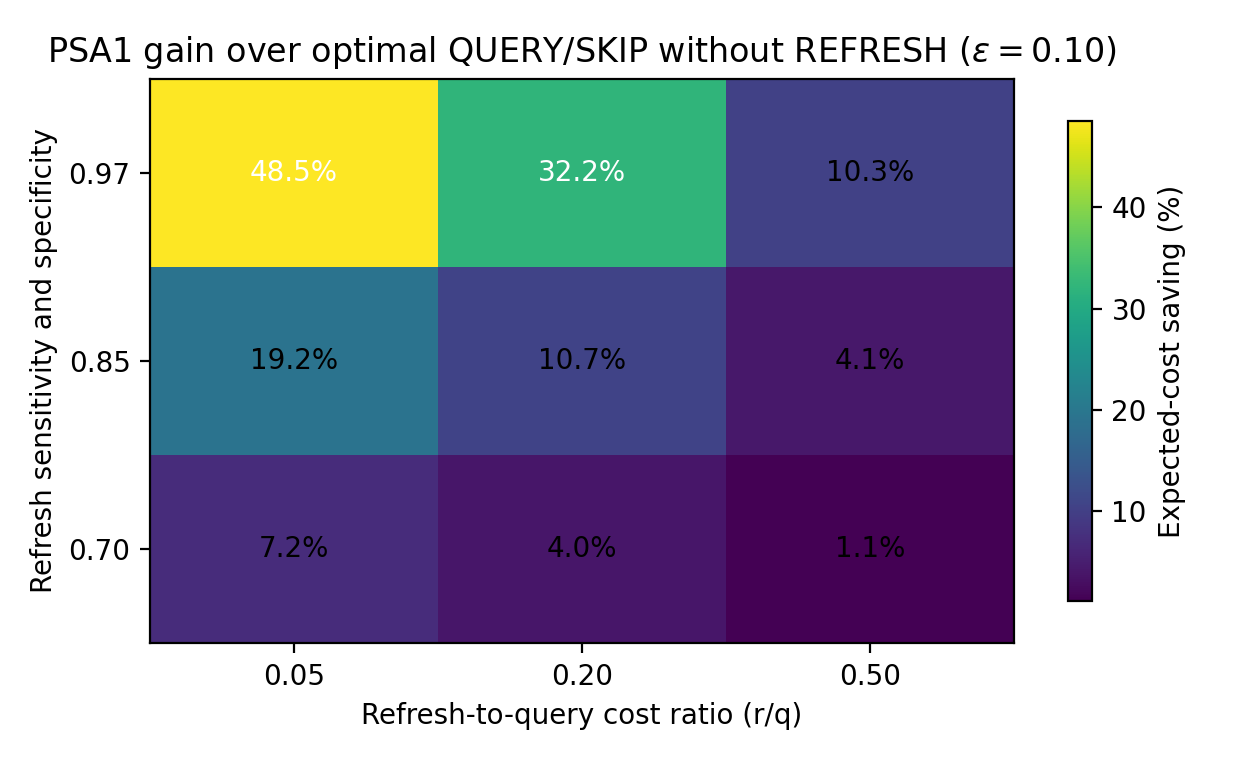
\includegraphics[width=\columnwidth]{results/figures/fig_refresh_sensitivity.png}
\caption{Additional PSA1 saving over optimal QUERY/SKIP without REFRESH at
$\varepsilon=0.10$ in the controlled synthetic factorial design.}
\label{fig:refresh_sensitivity}
\end{figure}

We also stress-test belief calibration by evaluating the policy under
true Bernoulli feasibility priors satisfying
$\mathrm{logit}(p_i^{\mathrm{true}})
=\mathrm{logit}(p_i^{\mathrm{nominal}})+\delta$,
while the policy continues to act on nominal beliefs. Across 375
instances, the model-consistent ($\delta=0$) conditional missed-resource
risk averaged 9.31\% over unsuccessful discoveries, and each instance
respected its own $\varepsilon$. For positive log-odds shifts
$\delta\in\{0.5,1.0,1.5\}$, the corresponding conditional risks became
14.54\%, 22.05\%, and 32.15\%. Since each instance has its own
$\varepsilon$ (mean 12.15\%), these aggregate numbers do not
constitute a single common risk constraint. The experiment shows that
the miss-risk assurance is contingent on calibrated beliefs and valid
observation models.

\subsection{Runtime and External Validity}
The median time to select the \emph{first} PSA1 action in a
skip-intensive stress family increased from 2.64~ms at $N=10$ to
0.150~s at $N=40$ and 1.239~s at $N=80$ in the unoptimized Python
implementation (eight independent instances per size). These values
concern online action selection, not exact enumeration of an entire
stochastic rollout tree; timings are hardware- and implementation-dependent.
The synthetic cases assume independent domain feasibility, calibrated
point beliefs unless explicitly perturbed, one requested resource,
and at most one refresh per domain. A complementary Alibaba GPU
trace-driven pilot uses measured workload and inventory inputs but
retains modeled domain federation, placement, and management costs;
its limited external validity is discussed separately.

\section{Discussion and Conclusion}
\label{sec:discussion}
The central idea is \emph{decision-sufficient} information: an
intent-management controller need not reconstruct every domain's full
state before making a suitable discovery decision. Instead, it can
actively balance expensive exact queries against cheaper but imperfect
knowledge refinement, under an explicit residual-risk budget.
\TODO{Discuss limitations: point-valued/calibrated beliefs,
independent domains, a single requested resource, at most one refresh
per domain, no resource contention, and model-to-trace transfer.}

% TODO: Insert a verified bibliography before submission. Bibliography
% is intentionally omitted from this compile-ready manuscript skeleton.
\end{document}
